\documentclass[11pt,a4paper]{article}

% ---------------------------------------------------------------------------
% Critical-window emergence of autocatalytic sets under reaction-channel
% quotienting.
%
% Author metadata: set the three macros below before submission.
% Build: see BUILD.md (pdflatex -> bibtex -> pdflatex -> pdflatex).
% ---------------------------------------------------------------------------
\newcommand{\PaperAuthor}{}
\newcommand{\PaperAffiliation}{}
\newcommand{\PaperDate}{September 14, 2026}

\usepackage[T1]{fontenc}
\usepackage[utf8]{inputenc}
\usepackage{lmodern}
\usepackage{microtype}
\usepackage[a4paper,margin=1.05in]{geometry}
\usepackage{amsmath,amssymb,amsthm,mathtools}
\usepackage{booktabs}
\usepackage{array}
\usepackage{enumitem}
\usepackage{xcolor}
\usepackage{graphicx}
\usepackage{tikz}
\usetikzlibrary{arrows.meta,positioning,calc}
\PassOptionsToPackage{hyphens}{url}
\usepackage{url}
\usepackage[colorlinks=true,linkcolor=blue!55!black,citecolor=blue!55!black,urlcolor=blue!55!black]{hyperref}

\setlist{itemsep=2pt,topsep=3pt}
\setlength{\emergencystretch}{1.5em}

\theoremstyle{plain}
\newtheorem{theorem}{Theorem}[section]
\newtheorem*{theorem*}{Main Theorem}
\newtheorem{proposition}[theorem]{Proposition}
\newtheorem{lemma}[theorem]{Lemma}
\newtheorem{corollary}[theorem]{Corollary}
\theoremstyle{definition}
\newtheorem{definition}[theorem]{Definition}
\newtheorem{example}[theorem]{Example}
\theoremstyle{remark}
\newtheorem{remark}[theorem]{Remark}

% Breakable typewriter identifiers for Lean names: \lean{Foo.bar_baz}
% (raw underscores permitted; break points after '.' and '_').
\makeatletter
\let\lean@us=_
\let\lean@end\relax
\DeclareRobustCommand{\lean}[1]{\begingroup\ttfamily\lean@scan#1\lean@end}
\def\lean@scan#1{\ifx#1\lean@end\endgroup\else\lean@char{#1}\expandafter\lean@scan\fi}
\def\lean@char#1{\ifx#1\lean@us\char`\_\allowbreak\else\ifx#1.\char`\.\allowbreak\else\ifx#1/\char`\/\allowbreak\else#1\fi\fi\fi}
\makeatother
% Lean declaration names attached to a statement, on their own ragged line.
\newcommand{\leanrefs}[1]{\par\nopagebreak{\small\raggedright\textup{Lean: #1.}\par}}
\newcommand{\conventional}{\par\nopagebreak{\small\raggedright\textup{Conventional proof; not formalised.}\par}}

\newcommand{\Prob}{\mathbb{P}}
\newcommand{\cl}{\mathcal{C}}
\newcommand{\qt}{\mathrm{qt}}
\newcommand{\spc}{\mathrm{sp}}
\newcommand{\eps}{\varepsilon}
\newcommand{\ee}{\mathrm{e}}
\newcommand{\Nat}{\mathbb{N}}
\newcommand{\Real}{\mathbb{R}}
\newcommand{\word}[1]{\mathtt{#1}}
\DeclareMathOperator{\RAF}{RAF}

\newcommand{\examplerows}{%
4 & 30 & 68 & 64 & 1.87500 & 0.171459 & 0.855743 \\
8 & 510 & 3076 & 3048 & 1.33858 & 0.125301 & 0.738244 \\
12 & 8190 & 81924 & 81828 & 1.20106 & 0.113174 & 0.699150 \\
16 & 131070 & 1835012 & 1834798 & 1.14297 & 0.108007 & 0.681131 \\
20 & 2097150 & 37748740 & 37748322 & 1.11112 & 0.105162 & 0.670811 \\
24 & 33554430 & 738197508 & 738196506 & 1.09091 & 0.103351 & 0.664089 \\
}


\title{Critical-window emergence of autocatalytic sets\\ under reaction-channel quotienting}
\author{\PaperAuthor\\ \PaperAffiliation}
\date{\PaperDate}

\begin{document}
\maketitle

\begin{abstract}
We determine the limiting probability that a reflexively autocatalytic and food-generated (RAF) set exists in the reversible binary-polymer model in the reaction convention used by the public generator of the finite-core theory of RAF emergence: two split descriptions $u+v\rightleftharpoons uv$ and $v+u\rightleftharpoons vu$ are identified precisely when $uv=vu$. Molecules are the nonempty binary words of length at most $n$, the food set consists of the six words of lengths one and two, and each molecule catalyses each reaction channel independently with probability $p_n$, one mark serving both directions. Let $f_n=p_n|J_n|$ be the mean number of channels catalysed by a molecule. For every sequence with $f_n/n\to\lambda>0$ the RAF probability converges to
\[
\Theta_{\qt}(\lambda)=S_{\qt}(1-\ee^{-\lambda})>0,
\]
where $S_{\qt}(a)$ is the probability that ordinary reversible closure of the food set is unbounded in an infinite field of independent canonical channels of openness $a$, and the probability of a RAF conditional on a catalysed food gateway converges to $S_{\qt}(1-\ee^{-\lambda})/(1-\ee^{-34\lambda})$. This resolves the bulk-factor problem left open in the companion paper on exact gateway scaling.

The quotient map preserves closures and RAF witnesses deterministically, but it does not preserve homogeneous Bernoulli ensembles: independent split marks project to heterogeneous OR marks, and a four-molecule example shows that the split and quotient RAF probabilities differ at every parameter. The proof therefore works in the quotient model throughout. A half-openness domination transfers a supplied-seed growth estimate from the split model through fibres of size at most two; a record-word argument proves that unbounded closure generates every fixed word at the original openness; a uniform finite-seed approximation gives continuity of $S_{\qt}$; an exact law for complete catalytic peeling histories connects static closure to the finite catalytic model; and a bounded-catalyst gateway bound closes the upper estimate. We also prove that $\Theta_{\qt}$ is nondecreasing and satisfies $S_{\spc}(1-\ee^{-\lambda/2})\le\Theta_{\qt}(\lambda)\le\min\{S_{\spc}(1-\ee^{-\lambda}),\,1-\ee^{-30\lambda}\}$, where $S_{\spc}$ is the split-position survival function, so that $\Theta_{\qt}(\lambda)\to0$ as $\lambda\downarrow0$ and $\Theta_{\qt}(\lambda)\to1$ as $\lambda\to\infty$. The main theorem and its dependencies are formalised in Lean~4 with no axioms beyond the classical foundation; the few hand-proved comparison results are labelled as such. The results concern structural autocatalysis, not kinetic or thermodynamic viability.
\end{abstract}

\noindent\textbf{Keywords.} autocatalytic sets; RAF theory; binary polymer model; reaction identity; quotient reaction networks; critical window; product measure; formal verification.

\medskip
\noindent\textbf{MSC 2020.} 60K35, 92E20, 05C80, 68V20.

\section{Introduction}\label{sec:intro}

Collectively autocatalytic sets were proposed by Kauffman~\cite{kauffman1986autocatalytic,kauffman1993origins}, following Eigen's hypercycle~\cite{eigen1971selforganization}, as a mechanism by which a random chemistry could support a self-sustaining metabolism without any single self-replicating molecule. Their combinatorial formalisation is the reflexively autocatalytic and food-generated set, or RAF, introduced by Steel~\cite{steel2000emergence} and developed with Hordijk~\cite{hordijk2004detecting,hordijk2012structure,hordijk2015algorithms,steel2019autocatalytic}; see~\cite{hordijk2010autocatalytic,hordijk2017chasing,hordijk2018life} for surveys. A RAF is a nonempty family of reactions that can generate all of its molecules from a prescribed food set and can find a catalyst for each of its reactions inside the resulting closure. RAF theory deliberately separates these structural requirements from any choice of reaction kinetics.

The standard test bed is the binary polymer model~\cite{kauffman1986autocatalytic,steel2000emergence,hordijk2004detecting}: molecules are binary words of length at most $n$, reactions are ligations and their reverse cleavages, the food set consists of the short words, and each molecule catalyses each reaction independently with a probability tuned so that a molecule catalyses on average $f_n$ reactions. Mossel and Steel~\cite{mossel2005random} showed that $f_n$ growing linearly in $n$ is the relevant scale for RAF occurrence, and simulations~\cite{hordijk2011required,hordijk2016variable} display a steep rise of the finite-$n$ RAF probability within a narrow range of $f_n/n$. A companion manuscript~\cite{criticalwindow2026} determined the limit on this scale for the textbook \emph{split-position} catalogue, in which a reaction is a product word together with a split position: if $f_n/n\to\lambda\in(0,\infty)$ then the RAF probability converges to $\Theta_{\spc}(\lambda)=S_{\spc}(1-\ee^{-\lambda})$, a continuous nondecreasing function with $0<\Theta_{\spc}(\lambda)\le1-\ee^{-36\lambda}<1$, where $S_{\spc}$ is the survival probability of an infinite reversible closure process. Thus the entire linear scale is a nontrivial critical window rather than a step.

\subsection*{Reaction identity}
The recent finite-core theory of RAF emergence of Varanasi and Korenaga~\cite{varanasi2026emergence} is accompanied by a public generator~\cite{varanasi2026repository} whose reaction catalogue differs from the split-position one: it compares displayed reactions and suppresses duplicates. The descriptions $\word A+\word{AA}\rightleftharpoons\word{AAA}$ and $\word{AA}+\word A\rightleftharpoons\word{AAA}$ are the same channel, while $\word A+\word B\rightleftharpoons\word{AB}$ and $\word B+\word A\rightleftharpoons\word{BA}$ remain distinct because their products differ. In general two split descriptions are identified exactly when their factors commute, $uv=vu$. A second companion manuscript~\cite{overlapgateway2026} worked in this quotient convention: it proved an exact overlap law for the RAF event, showed that for every $n\ge4$ exactly $34$ channels can fire from the six food words, derived the cap $\Prob(\RAF_n)\le1-(1-p_n)^{34|X_n|}$, and thereby the limit $1-\ee^{-34\lambda}$ for the gateway factor at $f_n=\lambda n$. It factorised the RAF probability as gateway probability times a gateway-conditioned bulk factor $B_n$, and left the limit of $B_n$, and the limit of the RAF probability itself, as its first open problem: ``it is open whether the two conventions have the same bulk limit.''

Deleting duplicate descriptions changes very little in the reaction count: the number of channels lost is $O(n^2 2^{n/3})$ out of $(n-2)2^{n+1}$ (Lemma~\ref{lem:count} and Remark~\ref{rem:count}). It nevertheless changes the random experiment, because in the quotient convention each surviving channel receives a \emph{single} Bernoulli mark per molecule, whereas in the split convention a commuting pair receives two. A four-molecule example (Example~\ref{ex:fixture}) shows that the two RAF probabilities differ at every parameter $p\in(0,1)$, even though every closure and every RAF witness corresponds exactly under the quotient map. An asymptotic count ratio therefore cannot identify the two limiting probabilities, and the split-position theorem of~\cite{criticalwindow2026} does not transfer by relabelling.

\subsection*{Main result}
We prove the critical-window law directly in the quotient model. Let $X_n$ be the nonempty binary words of length at most $n$, $J_n$ the quotient channels, $p_n=f_n/|J_n|$, and $P_n(p)$ the probability of a RAF under independent molecule--channel catalysis with parameter $p$. Let $S_{\qt}(a)$ be the probability that ordinary reversible closure of the food set is unbounded in an infinite field of independent canonical channels open with probability $a$ (Section~\ref{sec:model}).

\begin{theorem*}[Theorem~\ref{thm:main} below]
If $f_n/n\to\lambda>0$, then $0<p_n<1$ for all large $n$, and
\[
P_n(p_n)\longrightarrow\Theta_{\qt}(\lambda):=S_{\qt}(1-\ee^{-\lambda})>0,\qquad
B_n(p_n)\longrightarrow\frac{S_{\qt}(1-\ee^{-\lambda})}{1-\ee^{-34\lambda}},
\]
where $B_n(p)=P_n(p)/(1-(1-p)^{34|X_n|})$ is the gateway-conditioned bulk factor of~\cite{overlapgateway2026}.
\end{theorem*}

The theorem holds for every real sequence with the stated asymptotic intensity, not only $f_n=\lambda n$, and no assumption on a finite initial segment is needed. Section~\ref{sec:consequences} adds that $\Theta_{\qt}$ is nondecreasing, that
\[
S_{\spc}(1-\ee^{-\lambda/2})\ \le\ \Theta_{\qt}(\lambda)\ \le\ \min\{\Theta_{\spc}(\lambda),\,1-\ee^{-30\lambda}\},
\]
and that $\Theta_{\qt}(\lambda)\to0$ as $\lambda\downarrow0$ and $\Theta_{\qt}(\lambda)\to1$ as $\lambda\to\infty$; the sublinear and superlinear regimes are recovered as corollaries. The lower comparison is a Lean-verified consequence of the OR law; the upper comparisons and the endpoint values are short conventional arguments and are labelled as such.

\subsection*{Why the proof cannot be a transfer}
The quotient map $\pi_n$ from split descriptions to channels has fibres of size one or two. It preserves every stage of reversible closure and, for a fixed catalytic configuration, a split RAF exists if and only if a quotient RAF exists for the OR-projected marks (Lemma~\ref{lem:OR}). This deterministic equivalence is exact, but the OR projection of independent Bernoulli($p$) marks is independent with \emph{heterogeneous} parameters $1-(1-p)^{|\pi_n^{-1}(j)|}$, equal to $2p-p^2$ on the double fibres. The quotient model of the generator assigns $p$ on every channel. No homogeneous identity holds, and the two probability laws are different measures on the same channel set. The proof therefore establishes each analytic ingredient of the critical-window argument in the quotient model: the only object imported from the split model is one supplied-seed growth estimate, transferred through a coupling at half openness (Lemma~\ref{lem:bulk}), and that transfer is an inequality, not an identification.

\subsection*{Contributions}
\begin{enumerate}[label=\textbf{(\Alph*)},leftmargin=2.6em]
\item \textbf{Quotient critical-window law} (Theorem~\ref{thm:main}). The RAF probability of the quotient model converges at every positive intensity to $S_{\qt}(1-\ee^{-\lambda})>0$, and the gateway-conditioned bulk factor of~\cite{overlapgateway2026} converges to $S_{\qt}(1-\ee^{-\lambda})/(1-\ee^{-34\lambda})$.
\item \textbf{Deterministic versus distributional quotienting} (Lemma~\ref{lem:OR}, Example~\ref{ex:fixture}). Closures and RAF witnesses correspond exactly across the quotient; independent homogeneous laws do not. The correct projected law is the heterogeneous OR law, and a fibre coupling at reduced openness dominates it by a homogeneous one.
\item \textbf{Normalisation without enumeration} (Lemma~\ref{lem:count}). An arithmetic uniqueness argument for commuting words bounds the number of deleted descriptions by $n|X_{\lfloor(n-1)/2\rfloor}|$, so that $n|X_n|/|J_n|\to1$ and $p_n|X_n|\to\lambda$.
\item \textbf{Quotient analysis at the original parameter} (Sections~\ref{sec:richness}--\ref{sec:continuity}). Richness of unbounded closure, a uniform finite-seed approximation, and continuity of $S_{\qt}$ on $(0,1]$ are proved for the quotient field itself, with no auxiliary sprinkling field.
\item \textbf{Exact peeling-history law and sandwich} (Sections~\ref{sec:history}--\ref{sec:limit}). A complete-history replacement identity turns adaptive catalytic pruning into a fixed-pool static problem, giving the lower bound; a first-gateway argument with bounded catalysts gives the upper bound.
\item \textbf{Comparisons and regimes} (Section~\ref{sec:consequences}). Monotonicity, two-sided comparison with the split-position profile, the productive-gateway cap $1-\ee^{-30\lambda}$, endpoint limits, and the outer scaling regimes.
\item \textbf{Formal verification} (Appendix~\ref{app:formal}). The main theorem is the Lean~4 declaration \lean{RAFReactionQuotient.reaction_quotient_critical_window_resolution}, checked with warnings promoted to errors against the literal RAF predicate of the generator's model, with axiom closure $\{$\lean{propext}, \lean{Classical.choice}, \lean{Quot.sound}$\}$.
\end{enumerate}

\subsection*{Organisation}
Section~\ref{sec:model} fixes the model and states the main theorem. Section~\ref{sec:geometry} proves the OR law, the half-openness domination, and the channel count. Section~\ref{sec:bulk} states the supplied-seed estimate and transfers it. Sections~\ref{sec:richness} and~\ref{sec:continuity} prove richness, finite approximation, and continuity. Section~\ref{sec:history} converts static closure into catalytic RAFs through peeling histories, and Section~\ref{sec:limit} assembles the sandwich and proves Theorem~\ref{thm:main}. Section~\ref{sec:consequences} collects comparisons and regimes. Section~\ref{sec:interpretation} explains the consequences for reaction-network representation with a worked example, and Section~\ref{sec:discussion} discusses scope and open problems. Appendix~\ref{app:formal} gives the concordance between the numbered results and the Lean declarations.

\section{Model and main theorem}\label{sec:model}

\subsection{Molecules, channels, closure}
Let $\Sigma=\{\word A,\word B\}$ and
\[
X_n=\bigcup_{\ell=1}^{n}\Sigma^\ell,\qquad M_n=|X_n|=2^{n+1}-2,\qquad F=\Sigma\cup\Sigma^2 .
\]
We work with $n\ge2$; changing finitely many initial indices affects no limit below. The food set $F$ has six elements, $\word A,\word B,\word{AA},\word{AB},\word{BA},\word{BB}$.

A \emph{split description} is an ordered pair of nonempty words $(u,v)$ with $|u|+|v|\le n$, representing the reversible reaction $u+v\rightleftharpoons uv$. Write $R_n$ for the set of split descriptions; it is in bijection with the set of pairs (product word, split position), so $|R_n|=\sum_{\ell=2}^{n}(\ell-1)2^\ell=(n-2)2^{n+1}+4$. Two descriptions are \emph{equivalent} if their products are equal and their unordered factor pairs are equal. Write $J_n$ for the quotient and $\pi_n:R_n\to J_n$ for the quotient map. A nontrivial identification can only exchange the two factors, so it requires $uv=vu$; the canonical representative places the shorter factor first, and equal-length commuting factors are identical (Lemma~\ref{lem:comm}), so there is no residual ambiguity. This is exactly the channel set of the generator~\cite{varanasi2026repository}, formalised as \lean{RepositoryChannel}~$n$ in~\cite{overlapgateway2026}. The maps $\pi_n$ respect the inclusions $R_n\subseteq R_{n+1}$, and $J_\infty=\bigcup_nJ_n$ is well defined. Figure~\ref{fig:quotient} illustrates the quotient.

\begin{figure}[t]
\centering
\begin{tikzpicture}[>=Stealth,font=\small,
  desc/.style={draw,rounded corners=2pt,inner sep=3pt,minimum height=1.5em},
  chan/.style={draw,thick,rounded corners=2pt,inner sep=3pt,minimum height=1.5em,fill=black!4}]
% left block: commuting pair merges
\node[desc] (d1) at (0,1.1) {$\word A+\word{AA}\rightleftharpoons\word{AAA}$};
\node[desc] (d2) at (0,-0.1) {$\word{AA}+\word A\rightleftharpoons\word{AAA}$};
\node[chan] (c1) at (4.6,0.5) {channel $\{\word A,\word{AA}\}\rightleftharpoons\word{AAA}$};
\draw[->] (d1.east) -- (c1.west);
\draw[->] (d2.east) -- (c1.west);
\node[anchor=north,text width=4.4cm,align=center] at (2.3,-0.7) {fibre of size two:\\ split marks $\zeta_1,\zeta_2$, projected mark $\zeta_1\vee\zeta_2$};
% right block: non-commuting pair stays distinct
\node[desc] (e1) at (8.6,1.1) {$\word A+\word B\rightleftharpoons\word{AB}$};
\node[desc] (e2) at (8.6,-0.1) {$\word B+\word A\rightleftharpoons\word{BA}$};
\node[chan] (f1) at (12.2,1.1) {channel $\word{AB}$};
\node[chan] (f2) at (12.2,-0.1) {channel $\word{BA}$};
\draw[->] (e1.east) -- (f1.west);
\draw[->] (e2.east) -- (f2.west);
\node[anchor=north,text width=4.6cm,align=center] at (10.4,-0.7) {fibres of size one:\\ distinct products, marks unchanged};
\end{tikzpicture}
\caption{The commuting-factor quotient $\pi_n:R_n\to J_n$. Every fibre has size one or two. For a fixed catalyst, the projected catalytic mark of a channel is the OR of the split marks in its fibre; under independent Bernoulli($p$) split marks a double fibre is open with probability $2p-p^2$, whereas the quotient model assigns probability $p$ to every channel.}
\label{fig:quotient}
\end{figure}

For a channel family $A\subseteq J_n$ and a food cutoff $L\ge1$, let $\cl_{n,L}(A)$ be the smallest subset of $X_n$ containing $X_n\cap X_L$ and closed under both rules
\begin{equation}\label{eq:closure}
u,v\in\cl_{n,L}(A)\ \Longrightarrow\ uv\in\cl_{n,L}(A),\qquad
uv\in\cl_{n,L}(A)\ \Longrightarrow\ u,v\in\cl_{n,L}(A),
\end{equation}
whenever the channel of $(u,v)$ lies in $A$. Closure disregards catalysis: it records which molecules can be generated using the specified reactions from the supplied words. It treats availability as a set-valued property and does not count copies, so the multiplicity of a reactant is never a constraint. Write $\cl_n=\cl_{n,2}$ for closure from the food set.

\subsection{Random catalysis and the RAF event}
Let $\xi_{j,x}$, $j\in J_n$, $x\in X_n$, be independent Bernoulli variables with parameter $p\in[0,1]$. The event $\xi_{j,x}=1$ means that $x$ catalyses channel $j$ in both directions; no separate mark is assigned to cleavage. Food molecules may be catalysts.

\begin{definition}\label{def:raf}
A nonempty channel set $A\subseteq J_n$ is a \emph{RAF} if every endpoint of every channel in $A$ belongs to $\cl_n(A)$, and every $j\in A$ has a catalyst $x\in\cl_n(A)$ with $\xi_{j,x}=1$. Let $P_n(p)$ be the probability that at least one RAF exists.
\end{definition}

This is the closure-based RAF definition of~\cite{hordijk2004detecting,hordijk2011required} for a reversible reaction set and coincides with the predicate \lean{IsRevRAF} of~\cite{overlapgateway2026}; either side of a reversible channel may initiate its use, after which all its endpoints are available. The definition includes RAFs whose entire closure is food. The expected number of channels catalysed by one molecule is $f=p|J_n|$; following the generator we parametrise by $f$ and put $p_n=f_n/|J_n|$.

\subsection{The infinite canonical field and the survival function}
Independently of the catalytic model, for $a\in[0,1]$ give every $j\in J_\infty$ an independent Bernoulli($a$) \emph{open} mark, with product law $\Prob_a$. Let $\cl_\infty$ be the ordinary reversible closure of $F$ using the open channels, with no cap on word length. Define
\begin{equation}\label{eq:survival}
S_{\qt}(a)=\Prob_a\{\cl_\infty\ \text{contains words of arbitrarily large length}\}.
\end{equation}
Every membership assertion has a finite derivation, so the survival event is a countable combination of finite-coordinate events and is measurable. The restriction of the infinite field to $J_n$ is the homogeneous product law on $J_n$; we write $\Prob_a$ also for it. The field describes open channels, not catalytic assignments; its role is to name the limit.

\subsection{Gateways and the bulk factor}
A \emph{food gateway} is a channel with at least one side wholly contained in $F$. For $n\ge4$ there are exactly $34$ of them (Lemma~\ref{lem:gateways34}). Let $G_n$ be the event that some food gateway is catalysed by some molecule of $X_n$; its probability is $1-(1-p)^{34M_n}$. Since every RAF contains a catalysed gateway (Section~\ref{sec:limit}), $\{\RAF\}\subseteq G_n$, and the \emph{gateway-conditioned bulk factor} of~\cite{overlapgateway2026} is
\begin{equation}\label{eq:conditional}
B_n(p)=\Prob_p(\RAF\mid G_n)=\frac{P_n(p)}{1-(1-p)^{34M_n}},\qquad 0<p\le1 .
\end{equation}

\subsection{Main theorem}
\begin{theorem}[Quotient critical window]\label{thm:main}
Let $(f_n)$ be a real sequence with $f_n/n\to\lambda>0$ and put $p_n=f_n/|J_n|$. Then $0<p_n<1$ for all sufficiently large $n$, and
\begin{align}
P_n(p_n)&\longrightarrow\Theta_{\qt}(\lambda):=S_{\qt}(1-\ee^{-\lambda})>0,\label{eq:main}\\
B_n(p_n)&\longrightarrow\frac{S_{\qt}(1-\ee^{-\lambda})}{1-\ee^{-34\lambda}}.\label{eq:mainB}
\end{align}
\leanrefs{\lean{RAFReactionQuotient.reaction_quotient_critical_window_resolution}}
\end{theorem}

The Lean statement is the conjunction of four assertions: for all large $n$ the model parameter equals $f_n/|J_n|$ exactly (the totalising clamp used to define a measure for every real $f_n$ is eventually inactive); the RAF probability of the generator's actual finite catalogue converges to $S_{\qt}(1-\ee^{-\lambda})$; that limit is positive; and the actual gateway-conditioned factor converges to the displayed quotient. In particular, the conclusion is not a limit for a newly defined substitute event.

\begin{remark}
The theorem is an exact limit theorem. It provides no finite-size convergence rate, and the supplied-seed cutoff used in the proof is far too large to give one (Remark~\ref{rem:cutoff}). Figure~\ref{fig:finite} shows how slowly the finite-size channel openness approaches its limit, purely as a consequence of the normalisation.
\end{remark}

\section{Quotient geometry and normalisation}\label{sec:geometry}

\subsection{Closure projection and the OR law}
\begin{lemma}[Closure and OR projection]\label{lem:OR}
Every fibre of $\pi_n$ has size one or two. For an active split family $A'\subseteq R_n$, every stage of ordinary reversible closure of $A'$ coincides with the corresponding stage for $\pi_n(A')$. For split catalytic marks $\zeta_{r,x}$ define the projected marks
\[
\bar\zeta_{j,x}=\bigvee_{r\in\pi_n^{-1}(j)}\zeta_{r,x}.
\]
Then a split RAF exists for $\zeta$ if and only if a quotient RAF exists for $\bar\zeta$. If the split marks are independent Bernoulli($p$), the projected marks are independent with parameters
\begin{equation}\label{eq:OR}
q_j=1-(1-p)^{|\pi_n^{-1}(j)|}\in\{p,\,2p-p^2\}.
\end{equation}
\leanrefs{\lean{canonical_fibre_le_two}, \lean{split_closure_eq_quotient}, \lean{split_raf_iff_quotient}, \lean{fieldOR_independent}, \lean{fieldOR_closed_probability}, \lean{catalytic_OR_distribution}}
\end{lemma}

\begin{proof}
Only exchanging the two factors can give a second representative, so fibres have at most two members. Equivalent descriptions have exactly the same two chemical sides, so each closure stage in~\eqref{eq:closure} is unchanged by projection; induction on stages proves the closure assertion.

Project a split RAF together with its catalytic witnesses: the image family has the same closure and every image channel keeps a witness, so it is a quotient RAF for $\bar\zeta$. Conversely, given a quotient RAF $A$ for $\bar\zeta$, for each $j\in A$ choose a representative $r\in\pi_n^{-1}(j)$ whose split mark $\zeta_{r,x}$ realises one of the witnesses $x\in\cl_n(A)$ of $j$. The chosen representatives project onto $A$, so they have the same closure, and each has a catalyst in that closure; they form a split RAF. It is essential to choose the representative using the witness rather than fixing an arbitrary representative in advance.

A projected mark is zero precisely when every mark in its fibre is zero, giving~\eqref{eq:OR}. Distinct molecule--channel pairs involve disjoint sets of split coordinates, so the projected marks are independent.
\end{proof}

The OR law is a statement about the split ensemble viewed on the quotient channels. It is not the quotient model: the generator assigns probability $p$ to every channel, including the double fibres. The following example, checked by exact enumeration, shows that the difference is visible in the RAF probability itself.

\begin{example}[Split and quotient RAF probabilities differ]\label{ex:fixture}
Take molecules $\{\word A,\word{AA},\word{AAA},\word{AAAA}\}$, food $\{\word A,\word{AA}\}$, and the three split descriptions $(\word A,\word{AA})$, $(\word{AA},\word A)$, $(\word A,\word{AAA})$. The quotient has two channels, one with a double fibre. With independent Bernoulli($p$) marks on the three split descriptions for each of the four molecules, exact enumeration of the $2^{12}$ configurations gives a split RAF probability of $4077/4096$ at $p=1/2$; the OR-projected law reproduces this value exactly, as Lemma~\ref{lem:OR} predicts. The homogeneous quotient model with parameter $p=1/2$ on both channels gives $239/256=3824/4096$. At $p=1/3$ the values are $505585/531441$ and $5137/6561=416097/531441$. The events coincide configuration by configuration; the measures do not.
\end{example}

\subsection{Domination at reduced openness}
The OR law gives a one-directional comparison between homogeneous fields that is all the proof needs. Let $\Prob^{\spc}_b$ denote the law of independent Bernoulli($b$) marks on $R_n$ and $\Prob^{\qt}_a$ the law of independent Bernoulli($a$) marks on $J_n$. An event determined by the open channels is \emph{increasing} if it is preserved by opening more channels.

\begin{lemma}[Half-openness domination]\label{lem:half}
For $a\in[0,1]$ and every increasing event $E$ of the quotient field,
\begin{equation}\label{eq:half}
\Prob^{\spc}_{a/2}\{\bar\omega\in E\}\le\Prob^{\qt}_{a}(E),
\end{equation}
where $\bar\omega$ is the OR projection of the split field. The same holds with $a/2$ replaced by $1-\sqrt{1-a}$.
\leanrefs{\lean{product_increasing_mono}, \lean{OR_half_domination}, \lean{OR_sharp_domination}}
\end{lemma}

\begin{proof}
By Lemma~\ref{lem:OR} the projected field is an independent product with coordinate parameters $q_j\in\{a/2,\,1-(1-a/2)^2\}$, and $1-(1-a/2)^2=a-a^2/4\le a$. Couple the two product measures coordinatewise through independent uniform variables $U_j$, opening $j$ in the projected field when $U_j<q_j$ and in the quotient field when $U_j<a$. The projected configuration is then pointwise below the quotient configuration, and $E$ is increasing. For the sharper parameter, $1-(1-b)^2=a$ exactly when $b=1-\sqrt{1-a}$, and singletons have parameter $b\le a$.
\end{proof}

\subsection{Counting deleted descriptions}
\begin{lemma}[Commuting factors]\label{lem:comm}
Let $c(w)$ denote the integer whose binary expansion (with $\word A=0$, $\word B=1$ and leading zeros retained through the length) is $w$. If $uv=vu$ with $|u|=r$ and $|v|=s$, then $(2^r-1)c(v)=(2^s-1)c(u)$. Consequently, for a fixed word $u$ and a fixed length $s$, there is at most one word $v$ of length $s$ with $uv=vu$, and commuting factors of equal length are equal.
\leanrefs{\lean{commuting_factor_unique}, \lean{commuting_equal_length}}
\end{lemma}

\begin{proof}
Concatenation acts on codes by $c(uv)=2^{s}c(u)+c(v)$ and $c(vu)=2^{r}c(v)+c(u)$. Equating and rearranging gives the displayed identity. Since $2^r-1\neq0$, the code $c(v)$ is determined by $u$ and $s$, and a code with a prescribed length determines the word. If $r=s$ the identity gives $c(u)=c(v)$.
\end{proof}

\begin{lemma}[Deleted descriptions and normalisation]\label{lem:count}
Let $D_n=|R_n|-|J_n|$. Then
\[
|R_n|=(n-2)2^{n+1}+4,\qquad D_n\le n\,M_{\lfloor(n-1)/2\rfloor},\qquad \frac{nM_n}{|J_n|}\longrightarrow1 .
\]
\leanrefs{\lean{deletedKey_injective}, \lean{deleted_card_bound}, \lean{split_count_le_quotient_add_loss_bound}, \lean{quotient_normalization}}
\end{lemma}

\begin{proof}
The split count is $\sum_{\ell=2}^n(\ell-1)2^\ell$, which telescopes to the displayed formula. A deleted description is a noncanonical pair $(v,u)$ with $uv=vu$, $u\neq v$, and by Lemma~\ref{lem:comm} the factors have different lengths; say $|u|=r<|v|=s$. Associate to the deleted description the pair $(u,s)$. By Lemma~\ref{lem:comm} this association is injective. Because $r<s$ and $r+s\le n$ we have $r\le\lfloor(n-1)/2\rfloor$, so $u\in X_{\lfloor(n-1)/2\rfloor}$, while $s\le n$; this proves the bound. Since $M_k=2^{k+1}-2$, the bound gives $D_n/(nM_n)\le 2^{\lfloor(n-1)/2\rfloor+1}/(2^{n+1}-2)\to0$, and the exact split formula gives $|R_n|/(nM_n)\to1$. Subtracting and inverting gives the limit.
\end{proof}

\begin{remark}[Exact count]\label{rem:count}
By the Lyndon--Sch\"utzenberger theorem~\cite{lyndon1962equation,lothaire1997combinatorics}, $uv=vu$ with $u\ne v$ if and only if $u=w^a$, $v=w^b$ for a unique primitive word $w$ and $a\neq b$, which gives the exact closed form $D_n=\sum_{d\le n/3}P_d\lfloor(\lfloor n/d\rfloor-1)^2/4\rfloor$ with $P_d$ the number of primitive binary words of length $d$~\cite{overlapgateway2026}. The formal development uses only the elementary bound of Lemma~\ref{lem:count}, which suffices for normalisation and needs no theory of primitive words. The closed form agrees with exact enumeration for $n\le12$ (Table~\ref{tab:example}); for instance $D_{12}=96$ against the bound $12\cdot M_5=744$.
\end{remark}

Consequently the parameters in Theorem~\ref{thm:main} satisfy
\begin{equation}\label{eq:scaling}
p_n\longrightarrow0,\qquad p_nM_n\longrightarrow\lambda .
\end{equation}
Eventual positivity of $p_n$ follows from $f_n/n\to\lambda>0$ and eventual $p_n<1$ from $p_n\to0$. In Sections~\ref{sec:bulk}--\ref{sec:limit} we prove the RAF limit for every sequence $p_n\in[0,1]$ satisfying~\eqref{eq:scaling}; the general statement is \lean{quotient_critical_limit}, and \lean{quotientParameter_limits} discharges its premises for $p_n=f_n/|J_n|$.

\section{Uniform growth from a supplied seed}\label{sec:bulk}

The one quantitative input imported from the split-position development~\cite{criticalwindow2026} is a supplied-seed growth estimate. It is an unconditional theorem about ordinary reversible closure in the split field, proved there by a Peierls-type contour argument~\cite{peierls1936ising,grimmett1999percolation} on binary-word geometry; it makes no reference to RAFs or to any survival profile. We state it with its quantitative form so that its scope is explicit. For a cap $N$ and a food cutoff $L$, $\cl^{\spc}_{N,L}$ denotes reversible closure in $X_N$ of the supplied seed $X_L\cap X_N$ under the open split descriptions.

\begin{lemma}[Split supplied-seed estimate]\label{lem:splitbulk}
Fix $b>0$ and an integer $m\ge1$. There is $L>0$ such that for every $N\ge1$, under independent Bernoulli($b$) marks on $R_N$,
\begin{equation}\label{eq:splitbulk}
\Prob^{\spc}_b\bigl\{m\,|\cl^{\spc}_{N,L}|<(m-1)M_N\bigr\}\le\frac1m .
\end{equation}
\leanrefs{\lean{HordijkSteelThreshold.static_bulk_near_full}, \lean{static_bulk_deficit_bound}}
\end{lemma}

The quantitative statement behind Lemma~\ref{lem:splitbulk} is as follows. Put
\begin{equation}\label{eq:contour}
C_*=2\cdot7^{64}\cdot81,\qquad h_k=C_*(1-b^2)^k,\qquad \delta_k=\frac{h_k}{1-h_k}.
\end{equation}
For every $k$ with $h_k<1$, with $L=10k$, every $N\ge1$ and every integer $d\ge1$,
\begin{equation}\label{eq:deficit}
\Prob^{\spc}_b\bigl\{|\cl^{\spc}_{N,L}|+d\le M_N\bigr\}\le\delta_k+\frac{M_N\delta_k}{d}.
\end{equation}
The verified argument constructs a food-contracted word graph whose effective connections are realised by open two-reaction detours through short words. A contour of size $r$ separating a molecule from the seed has $kr$ disjoint detours available, so it fails with probability at most $(1-b^2)^{kr}$; the per-molecule contour envelope has at most $C_*^r$ members of size $r$; summing over $r\ge1$ bounds each molecule's probability of being cut off by $\delta_k$. If the root is not cut off, every molecule that is not cut off lies in its effective component, which lies in ordinary reversible closure. A union bound for the root and Markov's inequality for the number of cut-off molecules give~\eqref{eq:deficit}. The contour-envelope count and the disjoint-detour construction are theorems of the split development, not consequences of a numerical test; Appendix~\ref{app:formal} lists their modules. Only~\eqref{eq:deficit} is used here.

\begin{proof}[Derivation of Lemma~\ref{lem:splitbulk} from~\eqref{eq:deficit}]
Since $b>0$, choose $k\ge1$ with $\delta_k\le1/(m(m+1))$, take $L=10k$ and $d=\lfloor M_N/m\rfloor+1$. The event in~\eqref{eq:splitbulk} implies $|\cl^{\spc}_{N,L}|+d\le M_N$, while $M_N/d\le m$, so~\eqref{eq:deficit} gives probability at most $(m+1)\delta_k\le1/m$.
\end{proof}

\begin{lemma}[Quotient supplied-seed estimate]\label{lem:bulk}
For every $a_0>0$ and integer $m\ge1$ there is $L>0$ such that
\begin{equation}\label{eq:bulk}
\Prob_a\bigl\{m\,|\cl_{N,L}|<(m-1)M_N\bigr\}\le\frac1m\qquad\text{for all }a\in[a_0,1]\text{ and }N\ge1 .
\end{equation}
\leanrefs{\lean{quotient_supplied_seed_bulk}}
\end{lemma}

\begin{proof}
Apply Lemma~\ref{lem:splitbulk} at $b=a_0/2$ to obtain $L$. By Lemma~\ref{lem:OR} the closure of the projected split family equals the quotient closure of the projected marks, so the failure event in~\eqref{eq:bulk} is the projection of the failure event in~\eqref{eq:splitbulk}; it is a decreasing event. Lemma~\ref{lem:half} at every $a\ge a_0$ (its increasing complement, with $a_0/2\le a/2$) gives $\Prob_a\{\text{failure}\}\le\Prob^{\spc}_{a_0/2}\{\text{failure}\}\le1/m$. The same $L$ therefore works for all $a\ge a_0$ and all caps.
\end{proof}

This is the only transfer from split to quotient channels in the entire proof. No quotient contour enumeration is needed.

\begin{remark}[The cutoff is existential, not practical]\label{rem:cutoff}
The constant $C_*$ in~\eqref{eq:contour} makes the seed cutoff enormous. For $a_0=0.1$ and $m=10$ one needs $k$ with $C_*(1-b^2)^k<\eta/(1+\eta)$, $\eta=1/110$, i.e.\ $k\ge53667$ and $L=536670$; for $a_0=0.5$ the values are $k=2082$, $L=20820$. These are sufficient theoretical cutoffs, not convergence rates. A finite certified bracket $\Prob_a(H_{N,L})-1/m\le S_{\qt}(a)\le e_K(a)$ follows from the results below, but with these $L$ the lower bracket is not computable by enumeration, and we do not replace it by an unsupported numerical curve.
\end{remark}

\section{Richness at the original openness}\label{sec:richness}

We now work in the infinite quotient field of Section~\ref{sec:model} at a fixed openness $a>0$. The argument uses only the coordinates of that field; no auxiliary sprinkling is introduced.

The infinite field is realised on the coordinate set $\{(w,i)\}$ of split descriptions, indexed by product word and split position, and the quotient coordinates are the canonical indices $(w,i)\mapsto(w,i')$ that reverse the split position exactly when the two factors commute and the right factor is shorter. Canonicalisation preserves the product word and hence preserves every finite prefix of the field indexed by product length; its restriction to $J_n$ has the homogeneous product law on $J_n$.
\leanrefs{\lean{canonicalIndex_prefix}, \lean{infinite_quotient_restriction_map}}

\begin{lemma}[Survival generates every fixed word]\label{lem:rich}
For $a>0$ and every nonempty word $v$,
\[
\Prob_a\{\cl_\infty\ \text{is unbounded and}\ v\notin\cl_\infty\}=0 .
\]
\leanrefs{\lean{quotient_own_cap_record}, \lean{quotient_record_support}, \lean{quotient_cylinder_deficit}, \lean{quotient_missing_target_null}, \lean{quotient_target_ae}}
\end{lemma}

\begin{proof}
Expose channels by the length of their product. On unbounded closure there are arbitrarily long words $w$ generated using channels whose products have length at most $|w|$: take a finite derivation reaching beyond a given length and choose a longest word in it; that word is generated within its own cap. For each cutoff $B$, the first such \emph{record} above $B$, together with its finite prefix configuration and a fixed choice of a record word, gives a countable partition of the survival event into disjoint finite-prefix record events.

Write $v=v_1\cdots v_\ell$. From a record word $w$, append the target letters using the channels of
\[
w+v_1\rightleftharpoons wv_1,\qquad wv_1+v_2\rightleftharpoons wv_1v_2,\qquad\ldots,\qquad wv_1\cdots v_{\ell-1}+v_\ell\rightleftharpoons wv,
\]
and finally use $w+v\rightleftharpoons wv$ in the cleavage direction. Every letter is food, so if all of these channels are open then $v$ is generated. After canonicalisation the support contains at most $\ell+1$ distinct coordinates, each with product length strictly greater than $|w|$. Canonicalisation preserves the product, so every required coordinate lies outside the record prefix: the repair marks are \emph{fresh}. Conditional on any record event, the repair succeeds with probability at least $a^{\ell+1}$.

To use freshness without assuming independence between successive records, let $D$ be the event in the lemma and let $C$ be any event determined by a finite product-length prefix. Partition $D\cap C$ according to the first record above that prefix. On each piece the repair coordinates are fresh relative to the piece's prefix and the repair must fail (since $v\notin\cl_\infty$), so summing the disjoint pieces gives
\begin{equation}\label{eq:cylinderdeficit}
\Prob_a(D\cap C)\le(1-a^{\ell+1})\,\Prob_a(C).
\end{equation}
Finite-prefix events generate the product $\sigma$-algebra, so $D$ can be approximated in measure by such events $C$. Passing to the limit in~\eqref{eq:cylinderdeficit} gives $\Prob_a(D)\le(1-a^{\ell+1})\Prob_a(D)$, hence $\Prob_a(D)=0$.
\end{proof}

Survival therefore implies generation of every fixed finite seed with probability one. This is an almost-sure implication; it does not assert that every surviving configuration generates every word.

\section{Finite approximation and continuity}\label{sec:continuity}

For $L\ge1$ let $H_L$ be the event that every word of $X_L$ is eventually generated from $F$ in the infinite field, and let $H_{N,L}$ require generation within cap $N$, so that $H_{N,L}\uparrow H_L$ as $N\to\infty$. For $K\ge2$ let $E_K$ be the event that some word of length greater than $K$ is generated. A first escape from $X_K$ uses a ligation of two available words of length at most $K$, so its product has length at most $2K$; hence $E_K$ is determined by the channels of $J_{2K}$ even though closure is taken in the infinite field. Moreover $E_K\downarrow\{\cl_\infty\ \text{unbounded}\}$ as $K\to\infty$.

Write $h_{N,L}(a)=\Prob_a(H_{N,L})$ and $e_K(a)=\Prob_a(E_K)$. Each is a finite sum of terms $a^r(1-a)^{|J|-r}$ over configurations of a finite channel set and is therefore a polynomial in $a$. We have
\begin{equation}\label{eq:approx}
h_{N,L}(a)\uparrow\Prob_a(H_L)\ (N\to\infty),\qquad e_K(a)\downarrow S_{\qt}(a)\ (K\to\infty),
\end{equation}
and Lemma~\ref{lem:rich} gives $S_{\qt}(a)\le\Prob_a(H_L)$ for every $a>0$ and $L$.
\leanrefs{\lean{quotient_finite_seed_tendsto}, \lean{quotient_escape_tendsto}, \lean{quotientSurvival_le_seed}, \lean{continuous_quotient_event_probability}}

\begin{lemma}[Uniform seed approximation]\label{lem:seedapprox}
For every $a_0>0$ and integer $m\ge2$ there is $L>0$ such that
\begin{equation}\label{eq:seedapprox}
S_{\qt}(a)\le\Prob_a(H_L)\le S_{\qt}(a)+\frac1m\qquad(a\in[a_0,1]).
\end{equation}
\leanrefs{\lean{quotient_same_field_seed_mass}, \lean{quotient_uniform_seed_approximation}}
\end{lemma}

\begin{proof}
Choose $L$ from Lemma~\ref{lem:bulk}. In the same field at cap $N$, if $H_{N,L}$ occurs then the closure of the supplied seed $X_L\cap X_N$ is contained in the closure of $F$, because every seed word has already been generated from $F$. Consequently
\begin{equation}\label{eq:samefield}
\Prob_a(H_{N,L})\le\Prob_a\bigl\{m\,|\cl_{N,2}|\ge(m-1)M_N\bigr\}+\frac1m ,
\end{equation}
a union bound for two events in the same field; no independence is used. Fix $K$. For all sufficiently large $N$, a set of at least $(1-1/m)M_N$ words cannot fit inside $X_K$, so the mass event in~\eqref{eq:samefield} implies $E_K$. Letting $N\to\infty$ gives $\Prob_a(H_L)\le e_K(a)+1/m$, and letting $K\to\infty$ gives the upper bound in~\eqref{eq:seedapprox} by~\eqref{eq:approx}. The lower bound is Lemma~\ref{lem:rich}.
\end{proof}

\begin{proposition}[Continuity of the survival function]\label{prop:continuous}
$S_{\qt}$ is continuous at every $a\in(0,1]$ relative to $[0,1]$.
\leanrefs{\lean{quotientSurvival_tendsto}}
\end{proposition}

\begin{proof}
Let $a_i\to a>0$ and $\eps>0$. Choose $K$ with $e_K(a)<S_{\qt}(a)+\eps$. Since $e_K$ is a polynomial and $S_{\qt}(a_i)\le e_K(a_i)$, $\limsup_iS_{\qt}(a_i)\le S_{\qt}(a)+\eps$.

For the lower bound take $a_0=a/2$ and $m\ge2$ with $1/m<\eps$, and choose $L$ from Lemma~\ref{lem:seedapprox}. Choose $N$ with $h_{N,L}(a)>S_{\qt}(a)-\eps$, using~\eqref{eq:approx} and richness. Eventually $a_i\ge a_0$, so
\[
S_{\qt}(a_i)\ \ge\ \Prob_{a_i}(H_L)-\frac1m\ \ge\ h_{N,L}(a_i)-\frac1m ,
\]
and continuity of the polynomial $h_{N,L}$ gives $\liminf_iS_{\qt}(a_i)\ge S_{\qt}(a)-2\eps$. Let $\eps\downarrow0$. No uniform finite witness cap is asserted or needed.
\end{proof}

\section{From static closure to catalytic RAFs}\label{sec:history}

We return to the finite catalytic model on $J_n\times X_n$. For a realised catalytic matrix $\xi$ and a molecule set $C\subseteq X_n$ define the channels catalysed from $C$,
\[
A_\xi(C)=\{j\in J_n:\ \exists x\in C,\ \xi_{j,x}=1\}.
\]
Starting from all possible catalysts, \emph{peel} by
\begin{equation}\label{eq:peeling}
A_0=A_\xi(X_n),\qquad C_t=\cl_n(A_t),\qquad A_{t+1}=A_\xi(C_t).
\end{equation}
The channel sets decrease and stabilise by time $|J_n|$; write $A_*$ for the terminal set and $C_*=\cl_n(A_*)$ in this section. This is the standard RAF pruning algorithm of~\cite{hordijk2004detecting}.

\begin{lemma}[Terminal test]\label{lem:terminal}
Every RAF is contained in every $A_t$. Conversely, let $A^{\mathrm u}_*$ be the set of channels of $A_*$ all of whose endpoints lie in $C_*$. A RAF exists if and only if $A^{\mathrm u}_*\neq\varnothing$. In particular $|C_*|>6$ is sufficient for a RAF.
\leanrefs{\lean{quotient_raf_subset_peeling}, \lean{quotient_terminal_iff}, \lean{quotient_terminal_hasRAF}}
\end{lemma}

\begin{proof}
If $A$ is a RAF then $A\subseteq A_0$, and if $A\subseteq A_t$ then $\cl_n(A)\subseteq C_t$, so every catalyst of $A$ lies in $C_t$ and $A\subseteq A_{t+1}$. Conversely, removing from $A_*$ the channels with an endpoint outside $C_*$ does not change the closure, because a channel used in a derivation has all of its endpoints in the final closure; so $\cl_n(A^{\mathrm u}_*)=C_*$. Every channel of $A^{\mathrm u}_*$ has all endpoints in this closure and, by terminal stability $A_*=A_\xi(C_*)$, a catalyst in it. Hence a nonempty $A^{\mathrm u}_*$ is a RAF. If $|C_*|>6$ then some nonfood word is generated, so some channel of $A_*$ has all endpoints in $C_*$ and $A^{\mathrm u}_*\ne\varnothing$.
\end{proof}

The terminal test retains RAFs whose closure is food; the sufficient condition $|C_*|>6$ is used only for the lower bound and does not redefine the RAF event.

For a \emph{fixed} catalyst pool $C$ of size $k$, distinct channels are catalysed independently with probability
\begin{equation}\label{eq:qpool}
q(p,k)=1-(1-p)^k .
\end{equation}
The pools in~\eqref{eq:peeling} are adaptive, not fixed. The following identity is what permits the comparison.

\begin{lemma}[Complete-history replacement]\label{lem:history}
Fix an ordering of $X_n$ and let $I_k$ be its first $k$ elements. The entire finite sequence of channel sets in~\eqref{eq:peeling} has the same joint law if $A_\xi(C)$ is replaced at every step by $A_\xi(I_{|C|})$.
\leanrefs{\lean{quotient_column_history}, \lean{quotient_history_map}, \lean{quotient_pool_map}}
\end{lemma}

\begin{proof}
Fix a proposed decreasing history $A_0\supseteq A_1\supseteq\cdots\supseteq A_T$. Its prescribed pools are deterministic and nested: $D_0=X_n$ and $D_t=\cl_n(A_{t-1})$ for $t\ge1$. Put $s=1-p$ and $k_t=|D_t|$. For a single channel $j$, the column $(\xi_{j,x})_{x\in X_n}$ determines the first time $d$ at which $j$ leaves the history, namely the first $t$ with $A_\xi(D_t)\not\ni j$; the probability of each value is
\begin{equation}\label{eq:deathweight}
\begin{cases}
s^{k_0}, & d=0,\\[2pt]
s^{k_d}-s^{k_{d-1}}, & 1\le d\le T,\\[2pt]
1-s^{k_T}, & d=T+1\ \text{(catalysed from every pool)}.
\end{cases}
\end{equation}
Nestedness gives the middle line by subtraction: having no catalyst in $D_{d-1}$ implies having none in $D_d$. The event that the realised history equals the proposed one is the intersection over channels of the corresponding column constraints; columns are independent, so its probability is the product of the weights~\eqref{eq:deathweight}. Replacing the pools $D_t$ by the prefixes $I_{k_t}$ preserves their cardinalities and their nesting, hence every weight. Histories that are not decreasing have probability zero under both processes. Equality of the probabilities of all finite histories proves the claim. The proof does not condition the original columns on a random pool and then assert independence; it compares the two joint laws directly.
\end{proof}

\begin{lemma}[Static mass barrier]\label{lem:barrier}
If $6<k\le M_n$ then
\begin{equation}\label{eq:barrier}
\Prob_{q(p,k)}\bigl\{|\cl_{n,2}|\ge k\bigr\}\le P_n(p).
\end{equation}
\leanrefs{\lean{quotient_static_barrier}, \lean{quotient_mass_ge_static}}
\end{lemma}

\begin{proof}
Consider the prefix process of Lemma~\ref{lem:history} and suppose the fixed open family $A_\xi(I_k)$ generates at least $k$ molecules from food. It is contained in $A_0=A_\xi(X_n)$. Whenever it is contained in the current active family, the current closure has size at least $k$, so the next prefix pool contains $I_k$ and the family is contained in the next active family. By induction it is contained in every active family, so the terminal closure has at least $k>6$ elements and Lemma~\ref{lem:terminal} yields a RAF. Apply Lemma~\ref{lem:history} to transfer the probability to the original process, and note that $A_\xi(I_k)$ has the fixed-pool law~\eqref{eq:qpool}.
\end{proof}

For $m\ge2$ put $k_{n,m}=(m-1)\lfloor M_n/m\rfloor$. If $q\le q(p,k_{n,m})$ and $k_{n,m}>6$, monotonicity of product measures in the parameter gives
\begin{equation}\label{eq:nearlower}
\Prob_q\bigl\{m\,|\cl_{n,2}|\ge(m-1)M_n\bigr\}\le P_n(p),
\end{equation}
since the mass threshold implies $|\cl_{n,2}|\ge k_{n,m}$ and~\eqref{eq:barrier} applies.
\leanrefs{\lean{quotient_near_full_lower}}

\section{The probability sandwich}\label{sec:limit}

Assume $p_n\in[0,1]$ and~\eqref{eq:scaling}, and let $a=1-\ee^{-\lambda}\in(0,1)$. The elementary binomial limit gives
\begin{align}
q(p_n,M_n)&\longrightarrow a,\label{eq:poollimit}\\
q(p_n,k_{n,m})&\longrightarrow1-\ee^{-(1-1/m)\lambda}\qquad(m\ge2\ \text{fixed}),\label{eq:nearlimit}
\end{align}
because $\log(1-p_n)=-p_n+O(p_n^2)$ and $M_np_n^2=(M_np_n)p_n\to0$; the rounding in $k_{n,m}$ changes the exponent by a vanishing amount.
\leanrefs{\lean{generic_pool_limit}, \lean{generic_near_pool_mass}}

\subsection{Lower bound}
Fix $q\in(0,a)$ and $m\ge2$. Richness, finite seed approximation and Lemma~\ref{lem:bulk} imply
\begin{equation}\label{eq:massliminf}
\liminf_{n\to\infty}\Prob_q\bigl\{m\,|\cl_{n,2}|\ge(m-1)M_n\bigr\}\ \ge\ S_{\qt}(q)-\frac1m .
\end{equation}
Indeed, take the $L$ of Lemma~\ref{lem:bulk} for $a_0=q$, apply the same-field inclusion~\eqref{eq:samefield} at cap $n$, let $n\to\infty$ using $h_{n,L}(q)\uparrow\Prob_q(H_L)$, and use $\Prob_q(H_L)\ge S_{\qt}(q)$.

Choose $m$ so large that $q<1-\ee^{-(1-1/m)\lambda}$. By~\eqref{eq:nearlimit} and $k_{n,m}\to\infty$, inequality~\eqref{eq:nearlower} applies for all large $n$, so $\liminf_nP_n(p_n)\ge S_{\qt}(q)-1/m$. This holds for all sufficiently large $m$, hence $\liminf_nP_n(p_n)\ge S_{\qt}(q)$. Finally let $q\uparrow a$ and use Proposition~\ref{prop:continuous}:
\begin{equation}\label{eq:liminf}
\liminf_nP_n(p_n)\ge S_{\qt}(a).
\end{equation}

\subsection{Upper bound}
\begin{lemma}[The $34$ gateways]\label{lem:gateways34}
For $n\ge4$ there are exactly $34$ food gateways: four with a product of length two, fourteen with a product of length three, and sixteen with a product of length four. Every nonempty food-generated channel family contains a gateway.
\end{lemma}

\begin{proof}
A gateway has a side wholly in $F$. If the product side is in $F$ the product has length two and both factors are letters: four channels. Otherwise both factors are food words. Two letters and a letter with a dimer give the sixteen ordered length-three descriptions, among which $(\word A,\word{AA})\sim(\word{AA},\word A)$ and $(\word B,\word{BB})\sim(\word{BB},\word B)$ are the only commuting pairs, leaving fourteen channels. Two dimers give sixteen ordered descriptions; equal-length commuting factors are equal (Lemma~\ref{lem:comm}), so no two distinct descriptions merge and all sixteen are channels. A dimer with a trimer is not a gateway. For the second assertion, examine the first channel of the family that is enabled in a derivation of its own closure from food; its enabling side lies in $F$. If no derivation step is ever needed, all endpoints already lie in $F$ and any member is a gateway.
\end{proof}

The count $34$ was established for the generator's catalogue in~\cite{overlapgateway2026} by kernel evaluation, and the split-position count is $36$~\cite{criticalwindow2026}; the two missing channels are exactly the two identifications at product length three. A RAF supplies a catalyst for its gateway inside its own closure, so $\{\RAF\}\subseteq G_n$, as used in~\eqref{eq:conditional}.

Fix $K\ge2$. The closure of the full-pool active family $A_\xi(X_n)$ either escapes $X_K$, or it does not; in the second case every RAF, being contained in $A_0$ by Lemma~\ref{lem:terminal}, has closure inside $X_K$, so its gateway has a catalyst of length at most $K$. Therefore
\begin{equation}\label{eq:upper}
P_n(p_n)\le e_K\bigl(q(p_n,M_n)\bigr)+34\,M_K\,p_n .
\end{equation}
The first term uses the fixed-pool law~\eqref{eq:qpool} of $A_\xi(X_n)$ and the fact that a first escape from $X_K$ is determined by channels of product length at most $2K$; the second is a union bound over at most $34$ gateways and at most $M_K$ catalysts of bounded length. No independence is asserted after conditioning on failure to escape.
\leanrefs{\lean{quotient_bounded_seed_le}, \lean{quotient_raf_upper}}

For fixed $K$, continuity of the polynomial $e_K$, the limit~\eqref{eq:poollimit} and $p_n\to0$ give $\limsup_nP_n(p_n)\le e_K(a)$. Letting $K\to\infty$ and using~\eqref{eq:approx},
\begin{equation}\label{eq:limsup}
\limsup_nP_n(p_n)\le S_{\qt}(a).
\end{equation}
Together with~\eqref{eq:liminf} this proves the convergence in~\eqref{eq:main} for every sequence satisfying~\eqref{eq:scaling}.
\leanrefs{\lean{quotient_critical_limit}}

\subsection{Positivity, the actual catalogue, and the conditional limit}
The comparison of Lemma~\ref{lem:half} passes from the increasing finite events $E_K$ to their decreasing limit, so
\begin{equation}\label{eq:positivity}
S_{\qt}(a)\ \ge\ S_{\spc}(a/2)\ >\ 0\qquad(a>0),
\end{equation}
where $S_{\spc}$ is the split-position survival function of~\cite{criticalwindow2026}. Positivity of $S_{\spc}$ at every positive openness is a theorem of that development; it can also be read off Lemma~\ref{lem:splitbulk}: at a fixed positive openness, $m=2$ and each finite escape cutoff, a finite supplied seed survives with probability at least $1/2$, forcing the finitely many channels that generate that seed from $F$ to be open has positive probability, conditioning finitely many independent coordinates to be open can only increase supplied-seed survival, and on that event the food closure contains the seed closure.
\leanrefs{\lean{split_half_survival_le_quotient}, \lean{quotientSurvival_pos}, \lean{quotientTransitionLimit_positive}}

The probability $P_n(p)$ above is defined through a channel-indexed Boolean matrix. The generator, and the formal development of~\cite{overlapgateway2026}, describe a configuration by its family of catalyst subsets $(A_j)_{j\in J_n}$ and assign a configuration with $z$ present coordinates the weight $p^z(1-p)^{M_n|J_n|-z}$. The two descriptions are related by an explicit bijection under which the RAF predicates agree, and the weights of corresponding singletons coincide; summing them identifies the two finite probabilities.
\leanrefs{\lean{quotient_probability_eq_catalogue}}

Finally, the gateway coordinates are $34$ disjoint columns of $M_n$ independent marks, so
\[
\Prob_{p_n}(G_n)=1-(1-p_n)^{34M_n}\longrightarrow1-\ee^{-34\lambda}>0
\]
by~\eqref{eq:scaling}. Dividing the proved limit~\eqref{eq:main} by this positive limit gives~\eqref{eq:mainB}. Lemma~\ref{lem:count} discharges~\eqref{eq:scaling} for $p_n=f_n/|J_n|$, which completes the proof of Theorem~\ref{thm:main}.
\leanrefs{\lean{repository_gateway_critical_window}, \lean{repository_bulk_factor_critical_window}}

\section{Comparisons, caps, and regimes}\label{sec:consequences}

This section records what the proof gives beyond the limit itself. Results marked ``Lean'' are compiled declarations; those marked ``conventional'' are short hand proofs, and we keep the two carefully apart.

\subsection{Monotonicity}
\begin{proposition}\label{prop:mono}
$S_{\qt}$ is nondecreasing on $[0,1]$, and $\Theta_{\qt}(\lambda)=S_{\qt}(1-\ee^{-\lambda})$ is nondecreasing on $(0,\infty)$.
\leanrefs{\lean{quotientSurvival_mono}, \lean{quotientTransitionLimit_mono}}
\end{proposition}

\begin{proof}
Coordinatewise uniform coupling makes each finite escape event $E_K$ increasing in $a$; pass to the decreasing limit in $K$. Compose with the increasing map $\lambda\mapsto1-\ee^{-\lambda}$.
\end{proof}

\subsection{Two-sided comparison with the split-position model}
\begin{proposition}[Lower comparison]\label{prop:lower}
For $a\in[0,1]$, $S_{\spc}(1-\sqrt{1-a})\le S_{\qt}(a)$. Consequently $\Theta_{\spc}(\lambda/2)=S_{\spc}(1-\ee^{-\lambda/2})\le\Theta_{\qt}(\lambda)$.
\leanrefs{\lean{OR_sharp_domination}, \lean{split_sharp_survival_le_quotient}}
\end{proposition}

\begin{proof}
At split openness $b=1-\sqrt{1-a}$ a double fibre projects to OR probability $1-(1-b)^2=a$ and a singleton to $b\le a$, so Lemma~\ref{lem:half} in its sharp form dominates the projected finite escape events by the quotient ones; let $K\to\infty$. Since $1-\sqrt{\ee^{-\lambda}}=1-\ee^{-\lambda/2}$, the second statement follows.
\end{proof}

\begin{proposition}[Upper comparison]\label{prop:upper}
For $a\in[0,1]$, $S_{\qt}(a)\le S_{\spc}(a)$, hence $\Theta_{\qt}(\lambda)\le\Theta_{\spc}(\lambda)$.
\conventional
\end{proposition}

\begin{proof}
Couple the quotient field with a split field of the same openness by reading, for each channel, the split mark of its canonical representative. Representatives are distinct, so these are independent Bernoulli($a$) coordinates with the quotient law. Every open quotient channel then has an open split representative with the same two chemical sides, so every quotient derivation is pointwise a split derivation and $\cl^{\qt}_\infty\subseteq\cl^{\spc}_\infty$ configuration by configuration. Survival is preserved.
\end{proof}

The two comparisons say that the quotient profile is sandwiched between the split profile at half intensity and at full intensity. Whether $\Theta_{\qt}<\Theta_{\spc}$ strictly is discussed in Section~\ref{sec:discussion}. Neither comparison orders the gateway-normalised factors, whose denominators $1-\ee^{-34\lambda}$ and $1-\ee^{-36\lambda}$ differ.

\subsection{Gateway caps and endpoints}
\begin{proposition}[Caps]\label{prop:caps}
For every $\lambda>0$,
\[
\Theta_{\qt}(\lambda)\ \le\ 1-\ee^{-34\lambda}\qquad\text{and}\qquad \Theta_{\qt}(\lambda)\ \le\ 1-\ee^{-30\lambda}.
\]
The first bound combines two compiled statements, $P_n(p)\le1-(1-p)^{34M_n}$ from~\cite{overlapgateway2026} (\lean{repositoryRAFBernoulliProbability_le_gateway}) and the gateway limit of Theorem~\ref{thm:main}. The second follows from the conventional infinite-survival bound $S_{\qt}(a)\le1-(1-a)^{30}$.
\conventional
\end{proposition}

\begin{proof}
The first bound is immediate from the two cited limits. For the second, unbounded closure requires the generation of a nonfood word. Cleavage of a food word yields food words, so the first nonfood word ever produced is the product of a ligation whose two factors are food: a gateway with nonfood product. By Lemma~\ref{lem:gateways34} there are exactly $14+16=30$ such \emph{productive} gateways. If all thirty are closed, the closure remains equal to $F$. Their marks are independent, so $S_{\qt}(a)\le1-(1-a)^{30}$; substitute $a=1-\ee^{-\lambda}$.
\end{proof}

The finite RAF event retains food-only RAFs, so the $30$-gateway bound is a statement about infinite survival and about the limit, not about $P_n(p)$ at finite $n$, for which the $34$-gateway cap of~\cite{overlapgateway2026} is the correct statement. For the conditional limit, Proposition~\ref{prop:caps} gives
\[
\lim_nB_n(p_n)\ \le\ \frac{1-\ee^{-30\lambda}}{1-\ee^{-34\lambda}},\qquad
\limsup_{\lambda\downarrow0}\ \lim_nB_n(p_n)\ \le\ \frac{30}{34}.
\]
No equality and no small-$\lambda$ expansion is asserted.

\begin{proposition}[Endpoints]\label{prop:endpoints}
$S_{\qt}(0)=0$ and $S_{\qt}(1)=1$. Consequently $\Theta_{\qt}(\lambda)\to0$ as $\lambda\downarrow0$ and $\Theta_{\qt}(\lambda)\to1$ as $\lambda\to\infty$.
\conventional
\end{proposition}

\begin{proof}
At $a=0$ no channel is open and $\cl_\infty=F$. At $a=1$ every channel is open; by induction on length, a word of length $\ell+1$ is the ligation of its first letter with its length-$\ell$ suffix, both available, so every word is generated and closure is unbounded. The limit at $\lambda\downarrow0$ follows from the cap $1-\ee^{-34\lambda}$; the limit at $\lambda\to\infty$ follows from $S_{\qt}(1)=1$ and continuity of $S_{\qt}$ at $a=1$ (Proposition~\ref{prop:continuous}, Lean), since $1-\ee^{-\lambda}\to1$.
\end{proof}

\subsection{Outer scaling regimes}
For the two regimes outside the linear window the parameter $f_n/|J_n|$ need not lie in $[0,1]$ without an explicit assumption; $f_n/n\to\infty$ does not by itself give $f_n\le|J_n|$, and $f_n/n\to0$ does not give $f_n\ge0$. We therefore assume eventual validity.

\begin{corollary}[Sublinear and superlinear catalysis]\label{cor:outer}
Let $(f_n)$ satisfy $0\le f_n\le|J_n|$ for all $n$.
\begin{enumerate}[label=\textup{(\roman*)}]
\item If $f_n/n\to0$ then $P_n(p_n)\to0$.
\item If $f_n/n\to\infty$ then $P_n(p_n)\to1$.
\end{enumerate}
Part \textup{(i)} is a theorem of~\cite{overlapgateway2026}; part \textup{(ii)} is a conventional proof.
\leanrefs{\lean{sublinear_catalysis_forces_actual_repository_raf_vanishing} for (i)}
\end{corollary}

\begin{proof}
(i) is the gateway union bound $P_n(p_n)\le34M_np_n$ together with Lemma~\ref{lem:count}. For (ii) fix $c>0$. Eventually $f_n\ge cn$, so $p_n\ge cn/|J_n|=:p_n'$, and $P_n(\cdot)$ is nondecreasing in the parameter by coordinatewise coupling. Theorem~\ref{thm:main} applied to $f_n'=cn$ gives $\liminf_nP_n(p_n)\ge\Theta_{\qt}(c)$. Let $c\to\infty$ and apply Proposition~\ref{prop:endpoints}. No assumption $p_n\to0$ is used in (ii).
\end{proof}

\subsection{Independent heterogeneous catalysis}
The general limit theorem behind Theorem~\ref{thm:main} takes an arbitrary parameter sequence with $p_n\to0$ and $p_nM_n\to\lambda$ (\lean{quotient_critical_limit}). Combined with coupling it gives a robustness statement for heterogeneous but independent catalysis.

\begin{corollary}[Envelope bounds]\label{cor:envelope}
Keep the chemical model and let the coordinates $\xi_{j,x}$ be independent with $\Prob(\xi_{j,x}=1)=p_{n,j,x}$, where $\ell_n\le p_{n,j,x}\le u_n$ for all $j,x$ with $\ell_nM_n\to\lambda_-$ and $u_nM_n\to\lambda_+$ in $(0,\infty)$. Then
\[
S_{\qt}(1-\ee^{-\lambda_-})\ \le\ \liminf_n\Prob(\RAF_n)\ \le\ \limsup_n\Prob(\RAF_n)\ \le\ S_{\qt}(1-\ee^{-\lambda_+}).
\]
\conventional
\end{corollary}

\begin{proof}
Couple the three independent product fields through the same uniforms; RAF existence is increasing in the configuration, so $P_n(\ell_n)\le\Prob(\RAF_n)\le P_n(u_n)$. Both envelopes tend to zero with $\ell_nM_n,u_nM_n$ convergent, so the general limit theorem applies to each.
\end{proof}

The corollary covers uniformly small perturbations of the homogeneous law. It does not cover correlated catalytic marks, nor heterogeneity in the channel set itself; coordinate independence is essential to the coupling.

\section{Interpretation for reaction-network analysis}\label{sec:interpretation}

\subsection{Descriptions, channels, and probability laws}
The distinction between a reaction description and a reaction channel matters already in the smallest network. Consider one catalyst $x$ and the two descriptions of $\word A+\word{AA}\rightleftharpoons\word{AAA}$. If a database lists both, and a random-catalysis model assigns independent marks with probability $p$ to each listed description, then the chemically correct merged channel is catalysed by $x$ with probability $2p-p^2$: $3/4$ at $p=1/2$. If instead one first merges the descriptions and then assigns probability $p$ to the merged channel, the value is $1/2$. These are different probabilistic models on the same chemical channel, and Example~\ref{ex:fixture} shows that the difference propagates to the RAF probability. If, on the other hand, the two records are duplicate observations of the \emph{same} catalytic event, their marks coincide and the merged probability remains $p$; the OR formula with independent inputs must not be applied to duplicated observations without examining their dependence.

For a network analyst the immediate lesson is a preprocessing discipline: specify chemical equivalence of reaction descriptions first; determine which catalytic records represent independent events; and only then assign a probability law on the merged channels. In a biochemical database this requires preserving species identity, stoichiometry, direction, and compartment wherever these distinguish processes; $\word{AB}$ and $\word{BA}$ must remain distinct products. The binary-word quotient is a precise model of one such operation. It is not a universal equivalence rule for biochemical databases, and Theorem~\ref{thm:main} is a theorem about one model, not a transfer principle for every convention.

\subsection{A reproducible normalisation example}
Table~\ref{tab:example} and Figure~\ref{fig:finite} illustrate the normalisation used by the theorem, using exact counts only. The channel count $|J_n|$ is obtained for $n\le12$ by enumerating words and canonicalising commuting swapped factors, and for larger $n$ by the closed form of Remark~\ref{rem:count}; the two agree wherever both are available. The displayed openness $q_n=1-(1-p_n)^{M_n}$ is the exact full-pool channel probability~\eqref{eq:qpool} evaluated numerically; it is \emph{not} an estimate of the RAF probability, and no sampling is involved. Its limit is $1-\ee^{-\lambda}$, the argument of $S_{\qt}$ in Theorem~\ref{thm:main}. The finite-size correction is material: at $n=12$ and $\lambda=1$ the openness is $0.699$ against the limit $0.632$, because $nM_n/|J_n|$ approaches $1$ only like $1+2/(n-2)$. Any comparison between finite-$n$ simulations and the limiting profile must account for this normalisation before invoking $S_{\qt}$.

\begin{table}[t]
\centering
\caption{Exact channel census and finite-size openness. $M_n=|X_n|$, $|R_n|$ split descriptions, $|J_n|$ quotient channels; $q_n(\lambda)=1-(1-\lambda n/|J_n|)^{M_n}$ is the full-pool channel openness at $f_n=\lambda n$, whose limits are $1-\mathrm{e}^{-0.1}=0.095163$ and $1-\mathrm{e}^{-1}=0.632121$. Counts for $n\le12$ are by enumeration; larger $n$ use the closed form. Values are exact formula evaluations, not RAF probabilities.}
\label{tab:example}
\small
\begin{tabular}{rrrrrrr}
\toprule
$n$ & $M_n$ & $|R_n|$ & $|J_n|$ & $nM_n/|J_n|$ & $q_n(0.1)$ & $q_n(1)$\\
\midrule
\examplerows
\bottomrule
\end{tabular}
\end{table}

\begin{figure}[t]
\centering
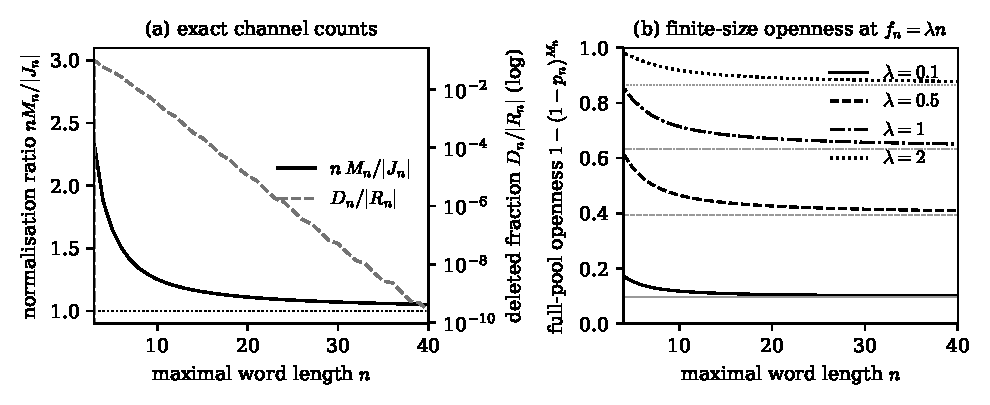
\includegraphics[width=\linewidth]{figures/finite_size.pdf}
\caption{(a) The normalisation ratio $nM_n/|J_n|$ (solid, left axis) and the fraction $D_n/|R_n|$ of split descriptions deleted by the quotient (dashed, right axis, logarithmic), from the exact counts. (b) The full-pool channel openness $1-(1-p_n)^{M_n}$ at $f_n=\lambda n$ for four intensities, with the limits $1-\mathrm{e}^{-\lambda}$ as thin horizontal lines. Both panels are exact evaluations; neither is a RAF probability.}
\label{fig:finite}
\end{figure}

\subsection{What the theorem does and does not say about chemistry}
Cooperative RNA catalytic networks~\cite{vaidya2012spontaneous} are an experimental motivation for studying the organisation of catalysis, and RAF theory has been used to interpret them~\cite{hordijk2014specificity}. Theorem~\ref{thm:main} does not calibrate such an experiment. The model has a fixed six-word food set, binary sequences, reversible set-valued availability, and independent catalytic marks; it omits concentrations, rates, inhibition, degradation, and any energy budget. Structural RAF existence therefore does not imply positive net flux, kinetic persistence, or thermodynamic feasibility; the extensions to dynamics and inhibition~\cite{hordijk2012extended} and to partitioned networks~\cite{smith2014partitioned} make these distinctions explicit. The intensity $\lambda$ is dimensionless and carries no implied rate or concentration unit. Applying the result to a particular chemical system would require a separate model-to-data calibration, which we do not attempt.

\section{Discussion}\label{sec:discussion}

\subsection*{What was resolved}
The companion paper~\cite{overlapgateway2026} isolated all unresolved linear-scale behaviour of the generator's model in the bulk factor $B_n$ and asked whether the split-position and quotient conventions share a bulk limit. Theorem~\ref{thm:main} determines $\lim B_n=S_{\qt}(1-\ee^{-\lambda})/(1-\ee^{-34\lambda})$, and Propositions~\ref{prop:lower} and~\ref{prop:upper} locate $\Theta_{\qt}$ between $\Theta_{\spc}(\lambda/2)$ and $\Theta_{\spc}(\lambda)$. The two profiles therefore have the same qualitative shape, a continuous nondecreasing curve from $0$ to $1$ across the whole linear scale, and the finite step conjecture of~\cite[Eq.~(21)]{hordijk2016variable} fails in the quotient convention for the same reason as in the split convention: no finite $\lambda$ separates limit zero from limit one.

\subsection*{Why a direct proof was necessary}
Every deterministic object transfers across the quotient: closures, RAF witnesses, caps, and record structure. What does not transfer is the measure. The failed shortcut, which we record because it is tempting, is to argue that the deleted fraction $D_n/|R_n|=O(n\,2^{-2n/3})$ is negligible and hence that the two homogeneous RAF probabilities have the same limit. The OR law shows the flaw: the split ensemble seen on the quotient channels is a \emph{different} product measure, with parameter $2p-p^2$ on every commuting pair, and Example~\ref{ex:fixture} shows that the difference reaches the RAF event. A negligible count ratio does not control a difference of measures whose supports are the same channel set. The proof therefore re-establishes richness, uniform approximation, continuity, and the sandwich in the quotient model, importing only one inequality from the split model.

\subsection*{Open problems}
\begin{enumerate}[label=\textup{(\arabic*)}]
\item \emph{Strictness.} Is $\Theta_{\qt}(\lambda)<\Theta_{\spc}(\lambda)$ for every $\lambda>0$? A conventional route couples the quotient field (canonical marks only) with the full split field, forces the noncanonical description $\word{AA}+\word A\rightleftharpoons\word{AAA}$ open and the other productive split gateways closed, so that the quotient is trapped at food while the split field escapes through $\word{AAA}$; a finite compatible repair support then generates a supplied seed from $\word{AAA}$, and Lemma~\ref{lem:splitbulk} gives positive split survival on this event. The exact geometry of the trap has been checked by enumeration (a repair support of $246$ split descriptions at seed cutoff $6$), but the formal docking of the coupling, the trap and the forcing step is incomplete, and we make no strictness claim. Strictness of the total survival probabilities would not by itself order the gateway-normalised factors.
\item \emph{Rates.} Theorem~\ref{thm:main} has no finite-size convergence rate, and the cutoffs of Remark~\ref{rem:cutoff} show that the present supplied-seed constant cannot supply a useful one. A contour estimate with a realistic constant, or a different amplification mechanism, would make finite certified brackets computable.
\item \emph{The value of $S_{\qt}$.} Nothing here identifies $S_{\qt}(a)$ beyond the bounds $S_{\spc}(1-\sqrt{1-a})\le S_{\qt}(a)\le\min\{S_{\spc}(a),1-(1-a)^{30}\}$ and the endpoints. Rigorous numerical bounds for $S_{\qt}$ or $S_{\spc}$ at a given openness are open.
\item \emph{Formalisation gaps.} The upper comparison, the productive-gateway cap, the endpoint values, and the superlinear regime are conventional proofs; each is short and should be formalised.
\item \emph{Beyond independence.} Corollary~\ref{cor:envelope} handles independent heterogeneous marks. Correlated catalysis, such as the specificity-structured catalysis of~\cite{hordijk2014specificity} or power-law catalysis distributions~\cite{hordijk2016variable}, is outside the product-measure method.
\end{enumerate}

\subsection*{Data and code availability}
The Lean sources are in the public repository \url{https://github.com/mmislan/Erdos} under \lean{proofs/RAFReactionQuotient/} (this paper), \lean{proofs/HordijkSteelThreshold/} (split-position development) and \lean{proofs/OverlapCorrectedRAF/} (quotient model and gateway). The exact census, the fixture enumeration of Example~\ref{ex:fixture}, the verification receipts, and the script producing Table~\ref{tab:example} and Figure~\ref{fig:finite} are under \lean{problem_workspaces/RAF_critical_window_reaction_quotient/} and \lean{key_results/RAFs/}.

\appendix
\section{Formal verification}\label{app:formal}

\subsection{The root declaration}
The main theorem is the Lean~4~\cite{demoura2021lean4} declaration
\begin{center}\small
\lean{RAFReactionQuotient.reaction_quotient_critical_window_resolution}
\end{center}
in \lean{proofs/RAFReactionQuotient/Resolution.lean}. Its universal parameters are $f:\Nat\to\Real$ and $\lambda:\Real$; its only hypotheses are $0<\lambda$ and $f(n)/n\to\lambda$. Its conclusion is the conjunction of four statements.
\begin{enumerate}[label=\textup{(\roman*)}]
\item For all large $n$ the model parameter equals $f(n)/|J_n|$ exactly.
\leanrefs{\lean{quotientParameter_eventually_exact}}
\item The generator's RAF probability converges to the survival probability of the infinite canonical field at openness $1-\ee^{-\lambda}$.
\leanrefs{\lean{repositoryRAFBernoulliProbability}, \lean{quotientTransitionLimit}, \lean{repository_critical_window}}
\item That limit is positive.
\leanrefs{\lean{quotientTransitionLimit_positive}}
\item The gateway-conditioned factor of~\cite{overlapgateway2026} converges to the quotient of the limit by $1-\ee^{-34\lambda}$.
\leanrefs{\lean{repositoryGatewayConditionedBulkProbability}, \lean{repository_bulk_factor_critical_window}}
\end{enumerate}
The finite RAF predicate, the channel type \lean{RepositoryChannel}, the Bernoulli catalogue, and the gateway factor are imported unchanged from the development of~\cite{overlapgateway2026}; the supplied-seed estimate is imported unchanged from the development of~\cite{criticalwindow2026}.

\subsection{Toolchain and audit}
Verification uses Lean \lean{v4.30.0} and the frozen Mathlib~\cite{mathlib2020} manifest checked into the repository (SHA-256 \lean{a8df0b60}\dots). The strict receipt records successful compilation of the root file with warnings promoted to errors, empty compiler output, and the authenticated declaration interface; the root source hash is \lean{ca3264cf}\dots\ and the receipt hash \lean{0f091921}\dots. The axiom closure of the root is $\{$\lean{propext}, \lean{Classical.choice}, \lean{Quot.sound}$\}$; there are no \lean{sorry}s, no problem-specific axioms, and no native unchecked computation. An independent freshness audit checks the source and compiled-artefact hashes of the $197$ recorded dependency modules and confirms that all $32$ local modules are covered by the root's dependency closure or by a successful supplementary receipt. The audit checks saved evidence and is not a substitute for the kernel check; formal verification establishes the encoded statement, and the model definitions of Section~\ref{sec:model} are what make that statement scientifically interpretable.

The supplementary module \lean{PublicationConsequences.lean} compiles Propositions~\ref{prop:mono} and~\ref{prop:lower} (\lean{quotientSurvival_mono}, \lean{quotientTransitionLimit_mono}, \lean{OR_sharp_domination}, \lean{split_sharp_survival_le_quotient}) with its own successful receipt. Propositions~\ref{prop:upper}, \ref{prop:caps} (second bound) and~\ref{prop:endpoints}, Corollary~\ref{cor:outer}(ii), and Corollary~\ref{cor:envelope} are conventional and are labelled as such in the text.

\subsection{Concordance}
Table~\ref{tab:formal} maps the results of the paper to their source modules. Modules in the main block are in \lean{proofs/RAFReactionQuotient/}, and the model, catalogue and gateway are in \lean{proofs/OverlapCorrectedRAF/}. The split supplied-seed estimate is in the directory \lean{proofs/HordijkSteelThreshold/}, in the modules \lean{StaticBulk} and \lean{StaticClosureMass}, whose geometric inputs are the modules
\leanrefs{\lean{WordMoleculeContourCount}, \lean{WordContourProbability}, \lean{WordContourMarginals}, \lean{WordEffectiveClosure}}

\begin{table}[ht]
\centering\small
\caption{Formal locations of the proof steps. Module names are files under the directories named in the text; declaration names are given beneath each result in the body of the paper.}
\label{tab:formal}
\begin{tabular}{>{\raggedright\arraybackslash}p{0.34\linewidth}>{\raggedright\arraybackslash}p{0.58\linewidth}}
\toprule
Result & Modules\\
\midrule
Lemma~\ref{lem:OR} (closure and OR projection) & \texttt{ClosureProjection}, \texttt{QuotientMap}, \texttt{SplitAdapter}, \texttt{Fibres}, \texttt{Surjectivity}, \texttt{CapCompatibility}, \texttt{ORLaw}, \texttt{ORDistribution}, \texttt{CatalyticOR}\\
Lemma~\ref{lem:half} (domination) & \texttt{ProductDomination}, \texttt{PublicationConsequences}\\
Lemmas~\ref{lem:comm}--\ref{lem:count} (count, normalisation) & \texttt{CommutingUniqueness}, \texttt{CountLoss}, \texttt{Counts}, \texttt{SourceParameters}\\
Lemma~\ref{lem:splitbulk} (split supplied seed) & \texttt{HordijkSteelThreshold/StaticBulk}, \texttt{StaticClosureMass}\\
Lemma~\ref{lem:bulk} (quotient supplied seed) & \texttt{SeedBulk}\\
Infinite law, records, Lemma~\ref{lem:rich} & \texttt{InfiniteSource}, \texttt{InfiniteDock}, \texttt{Richness}\\
\eqref{eq:approx}, Lemma~\ref{lem:seedapprox}, Prop.~\ref{prop:continuous} & \texttt{FiniteApproximation}, \texttt{EventContinuity}, \texttt{SeedApproximation}, \texttt{SurvivalContinuity}\\
Lemmas~\ref{lem:terminal}--\ref{lem:barrier} (peeling) & \texttt{History}, \texttt{Terminal}, \texttt{PoolLaw}, \texttt{SourceBounds}\\
Section~\ref{sec:limit} (sandwich, positivity, catalogue) & \texttt{PoolLimits}, \texttt{CriticalLimit}, \texttt{SurvivalPositive}, \texttt{CatalogueBridge}, \texttt{Resolution}\\
Propositions~\ref{prop:mono}, \ref{prop:lower} & \texttt{PublicationConsequences}\\
\bottomrule
\end{tabular}
\end{table}

\subsection{Reproduction}
From the repository root, with the pinned Lean working directory enforced by the wrapper (line breaks are for display only):
\begin{quote}\footnotesize\ttfamily\raggedright
.venv/Scripts/python.exe scripts/verify\_proof.py\\
\ \ proofs/RAFReactionQuotient/Resolution.lean --timeout 900\\
\ \ --declaration RAFReactionQuotient.reaction\_quotient\_critical\_window\_resolution\\
\ \ --output problem\_workspaces/RAF\_critical\_window\_reaction\_quotient/\\
\ \ \ \ \ \ \ \ \ \ verification/Resolution.verify.json\\[3pt]
.venv/Scripts/python.exe\\
\ \ problem\_workspaces/RAF\_critical\_window\_reaction\_quotient/audit\_resolution.py
\end{quote}
The first command recompiles the root and its dependency closure and writes a receipt; the second replays the freshness audit. The table and figure of Section~\ref{sec:interpretation} are produced by \lean{make_figures.py} in the manuscript source directory, which also re-derives the census of the workspace pilot and asserts agreement between enumeration and closed form. No dependency update is needed to reproduce the proof.

{\small
\bibliographystyle{plain}
\bibliography{refs}
}

\end{document}
